\documentclass[dvips,12pt,a4paper]{report}
\usepackage[dvips]{graphicx}
%\usepackage[dvips]{color}
\usepackage[latin1]{inputenc}
\usepackage[T1]{fontenc}
%\usepackage{ae,aecompl}
\usepackage{pslatex}
%\usepackage[portuges]{babel}
\usepackage{hyperref}
\usepackage[footnotesize]{caption}
\usepackage{subfigure}
\usepackage{amsmath}
\usepackage{amssymb}
\usepackage{bm}
\usepackage{lscape}
\usepackage{multicol}
\usepackage{longtable}
\usepackage{rotating}
\usepackage{color}
\usepackage{colortbl}
\usepackage{fancyheadings} % entete et bas de page
\usepackage{natbib}
\usepackage[left=3cm,right=2.5cm,top=3cm,bottom=3cm]{geometry}
\usepackage{setspace}
%\usepackage{natbib}
%\singlespacing
\onehalfspacing
%\doublespacing
%pour hautdepage
%[] page im paire {} page impaire
\lhead[\fancyplain{}{\sffamily \leftmark}]{}
\chead{}
\rhead[]{\fancyplain{}{\sffamily \rightmark}}
\cfoot{}
%\pagestyle{fancy}


\usepackage{graphicx}
%\usepackage{txfonts}




\title{ \huge {\textbf{Annual PDA Progress Report \\
Year One }}  
\\ [2cm]
\LARGE {Stellar parameters for M dwarfs: the link to exoplanets}}

\author{\\
\\
Vasco de Matos Ferreira Mendes Neves \\
\\
\\
Centro de Astrof\'{\i}sica da Universidade do Porto (CAUP) \\
Laboratoire d'Astrophysique de L'Universit\'e de Grenoble (LAOG)\\
\\
\\
\\
Orientation by:\\
Nuno Santos (CAUP) \\ Xavier Delfosse (LAOG)}
\date{September 2010}

\begin{document}
\pagenumbering{roman}
\maketitle

\begin{abstract}
I will present, in this report, an overview of the plan of the thesis that is going to be executed in the next two years. My Ph.D. program is about M stars and the challenges of determining its parameters (namely, metallicity, effective temperature, surface gravity, microturbulence, mass, and radius) with good precision, when compared with present state-of-the-art studies. The main goal is to use these parameters, with a special emphasis on metallicity, to study the star-planet connection, as well as to improve the planetary parameters, using the data from planet detection techniques, such as radial velocity and transit detection. In chapter one I will make a short introduction to the topic at hand, followed, in chapter two, by a description of the state of the art. Then, in chapter three, I will detail the general goals of my project.  Finally, in chapter four, I will describe the different methods, with their pros and cons, that might be used to achieve my goals. %The goals will be detailed in Chapter four.  %In the last chapter, I will do a brief resume of the work that was done up to this point.

%DUVIDA linha 1 - two or three years? ; 	Trocar chapter 3 pelo 4 e apagar o chapter 5?

\end{abstract}

\tableofcontents
\newpage
\pagenumbering{arabic}
\renewcommand*\thesection{\arabic{section}}
%Introduction%%%%%%%%%%%%%%%%%%%%%%%
%\setcounter{section}{0}
\section{Introduction}

%\addcontentsline{toc}{chapter}{Introduction}
\cfoot{ { \thepage} }
%\pagestyle{fancy}

M dwarfs are the faintest, smallest, and coldest of all stars in the main sequence (MS). They are situated at the bottom right corner of the HR diagram (see Fig. \ref{hrdiagram}). %For a long time, they  discreet and uninteresting but, in fact, they are very important: 
More than two thirds of the stars in the galaxy are M dwarfs, and they make up the majority of its baryonic matter \citep{Chabrier-2003}. Despite this, they are one of the least understood stellar types: M dwarfs are hard to study, due to their intrinsic faintness and complex spectra. Therefore, new studies regarding this faint component are needed, in order to get a more realistic model of the Galaxy.

\begin{figure}[h]
\centering
\includegraphics[height=10cm]{pics/HR_diagram.eps}
\caption[] {The HR Diagram. The M dwarfs are situated at the bottom right corner of the main sequence.}
\label{hrdiagram}
\end{figure}

The study of M stars is also increasingly important in the context of planet formation around very low mass stars. Some theoretical models %on the formation of planets  on M dwarfs 
predict that the formation of giant planets is seriously inhibited around the less massive stars ($M_{*} < 0.4 M_{\odot}$) (e.g. \citeauthor{Laughlin-2004} \citeyear{Laughlin-2004}; \citeauthor{Ida-2005} \citeyear{Ida-2005}). According to them, the formed rocky or ice cores do not have enough time to get a gas envelope and become super-earths or ice giants instead. Others suggest that the proto-planets may have enough time to grow and to accrete the gas envelope before the disk vanishes, by invoking migration and faster accretion (e.g. \citeauthor{Alibert-2005} \citeyear{Alibert-2005}). Alternatively, \citet{Boss-2006a}, and \citet{Boss-2006b} show that the disk instability hypothesis can also play a role in the formation of planets around M dwarfs. Indeed, an increasingly number of planets are being detected around these stars and they show that most planets have, on average, a lower mass than those found on FGK stars, the majority being neptunians and super-earths (e.g. \citeauthor{Bonfils-2007} \citeyear{Bonfils-2007}; \citeauthor{Udry-2007} \citeyear{Udry-2007}). %However, it is not yet clear, due to a lack of high quality metallicity ([Fe/H]) measurements, if the root cause of the deficit of Jovian planets around M stars is due mainly to stellar mass or metallicity \citep{Johnson-2009}.

%NOTA: Confirmar se o Alibert-2005 se aplica �s M dwarfs!!!! Penso que � geral

In the last few years there has been an increased interest in studying M dwarfs, motivated by the fact that is easier to detect lower mass planets around these stars, with the assumed goal of finding the first earth-class ($\sim1 M_{\oplus}$) exoplanet. In fact, the M stars mass and radius (between 0.6 to 0.08 $M_{\odot}$, and 0.6 to 0.1 $R_{\odot}$ respectively), imply that the reflex velocities induced by planets around them, as well as the transit depths, are considerably larger, when compared to the same effects induced in the more massive, and better studied, FGK stars. Moreover, the habitable zone in these stars are situated in tighter orbits, which makes the detection of planets in this area easier with radial velocity and transit techniques, as both have their best sensitivity closer to the host star \citep{Nutzman-2008}.

The number of detected exoplanets is increasing fast. According to 'The Extrasolar Planets Encyclopaedia'\footnote{http://exoplanet.eu/}, 490 planet candidates now exist (as of 20/09/2010). The growing number of exoplanets, as well as a copious amount of high S/N, high-resolution spectra from their host stars, available from radial velocity surveys, allow the statistical analysis of their properties as well as the properties of their host stars (for a review see \citeauthor{Udry-2007} \citeyear{Udry-2007}). In fact, these studies are providing important constrains for the models of formation and evolution of these systems. 

For M dwarfs, however, the derivation of accurate parameters is not an easy task. The observational spectra of these stars gets more and more complex as the stellar subtype increases, due to the increasing presence of millions of weak molecular lines (TiO, VO, H2O, CO, FeH, etc), that blend with other atomic lines and depress the continuum, making the spectral analysis difficult (e.g. \citeauthor{Gustafsson-1989} \citeyear{Gustafsson-1989}). For late M dwarfs, the atomic line analysis becomes impossible. One alternative would be to use high-resolution spectral synthesis (e.g. \citeauthor{Valenti-1998} \citeyear{Valenti-1998}), but this method does not yet reproduce the fine details of high-resolution spectra of M stars due to incomplete knowledge about the molecular line transitions, and opacities (e.g. \citeauthor{Bean-2006} \citeyear{Bean-2006}). The lack of good atmospheric models also affects the direct measurement of atomic and molecular lines, limiting the accuracy of their determinations. Other studies explore different approaches, that include, for example, the use of low resolution spectra to determine molecular indices dependent on metallicity or effective temperature (e.g. \citeauthor{Woolf-2006} \citeyear{Woolf-2006}), or very accurate broadband photometry in multiple wavelengths such as IRFM or MOITE \citeauthor{Casagrande-2008} \citeyear{Casagrande-2008}, in order to determine accurate values of metallicity or/and effective temperature, thus allowing the calibration of these parameters within a certain region of validation. The different techniques, their advantages and drawbacks, will be described in detail in Chapter 4.

%In the context of fundamental parameter determination, the most important are metallicity and effective temperature.

%Regarding metallicity, for example, several calibrations exist, using different techniques, but no consensus has yet been reached (see e.g. xxx,yyy,zzz). 


%One of the most striking example of the star-planet connection is the statistical difference of the value of metallicity between stars with and without giant planets: the probability of finding one of these planets is higher in stars with high metal content (e.g. xxx,yyy,zzz). Regarding M dwarfs, however, this relation is not clear. 

%\citeauthor{} \citeyear{}

%In parallel with the exoplanet detection and characterization, several studies appear regarding the characterization of the host stars (e.g. xxx...). 


\section{State of the Art}

An increasingly number of exoplanets are being detect around M dwarfs (e.g. \citeauthor{Delfosse-1998} \citeyear{Delfosse-1998}; \citeauthor{Bonfils-2007} \citeyear{Bonfils-2007}; \citeauthor{Mayor-2009} \citeyear{Mayor-2009}). There are now about thirty known exoplanets orbiting these stars, according to 'The Extrasolar Planet Encyclopeadia'. In the last few years, efforts have been done to characterize the stellar parameters of M dwarfs, trying to get more precise values of metallicity, temperature, mass, radius, and surface gravity using different methods. These values will be very important in constraining the models of formation and evolution of planetary systems, thus giving a better understanding of the physics at play. The determination of precise parameters for the stars will also help improving the precision of the planet's mass and radius, with the aid of the data coming from transits.

\subsection{Metallicity \& Temperature}

One of the most remarkable correlations found so far for FGK stars that is improving the understanding of the processes of planetary formation is related to the host star: the stars with higher metallicity content have, on average, a higher probability of hosting Jovian class planets (\citeauthor{Gonzalez-1997} \citeyear{Gonzalez-1997}; \citeauthor{Santos-2001a} \citeyear{Santos-2001a}; \citeauthor{Fischer-2005} \citeyear{Fischer-2005} - see Fig. \ref{fehhist}). Whether or not this correlation extends to the cooler M dwarfs is still highly controversial and requires very precise measurements. Interestingly, this correlation is likely not observed for FGK stars orbited by Neptune or Super-Earth type planets ( \citeauthor{Sousa-2008} \citeyear{Sousa-2008}; \citeauthor{Bouchy-2009} \citeyear{Bouchy-2009}). Whether or not the same happens on M dwarfs remains to be seen.

\begin{figure}[h]
\centering
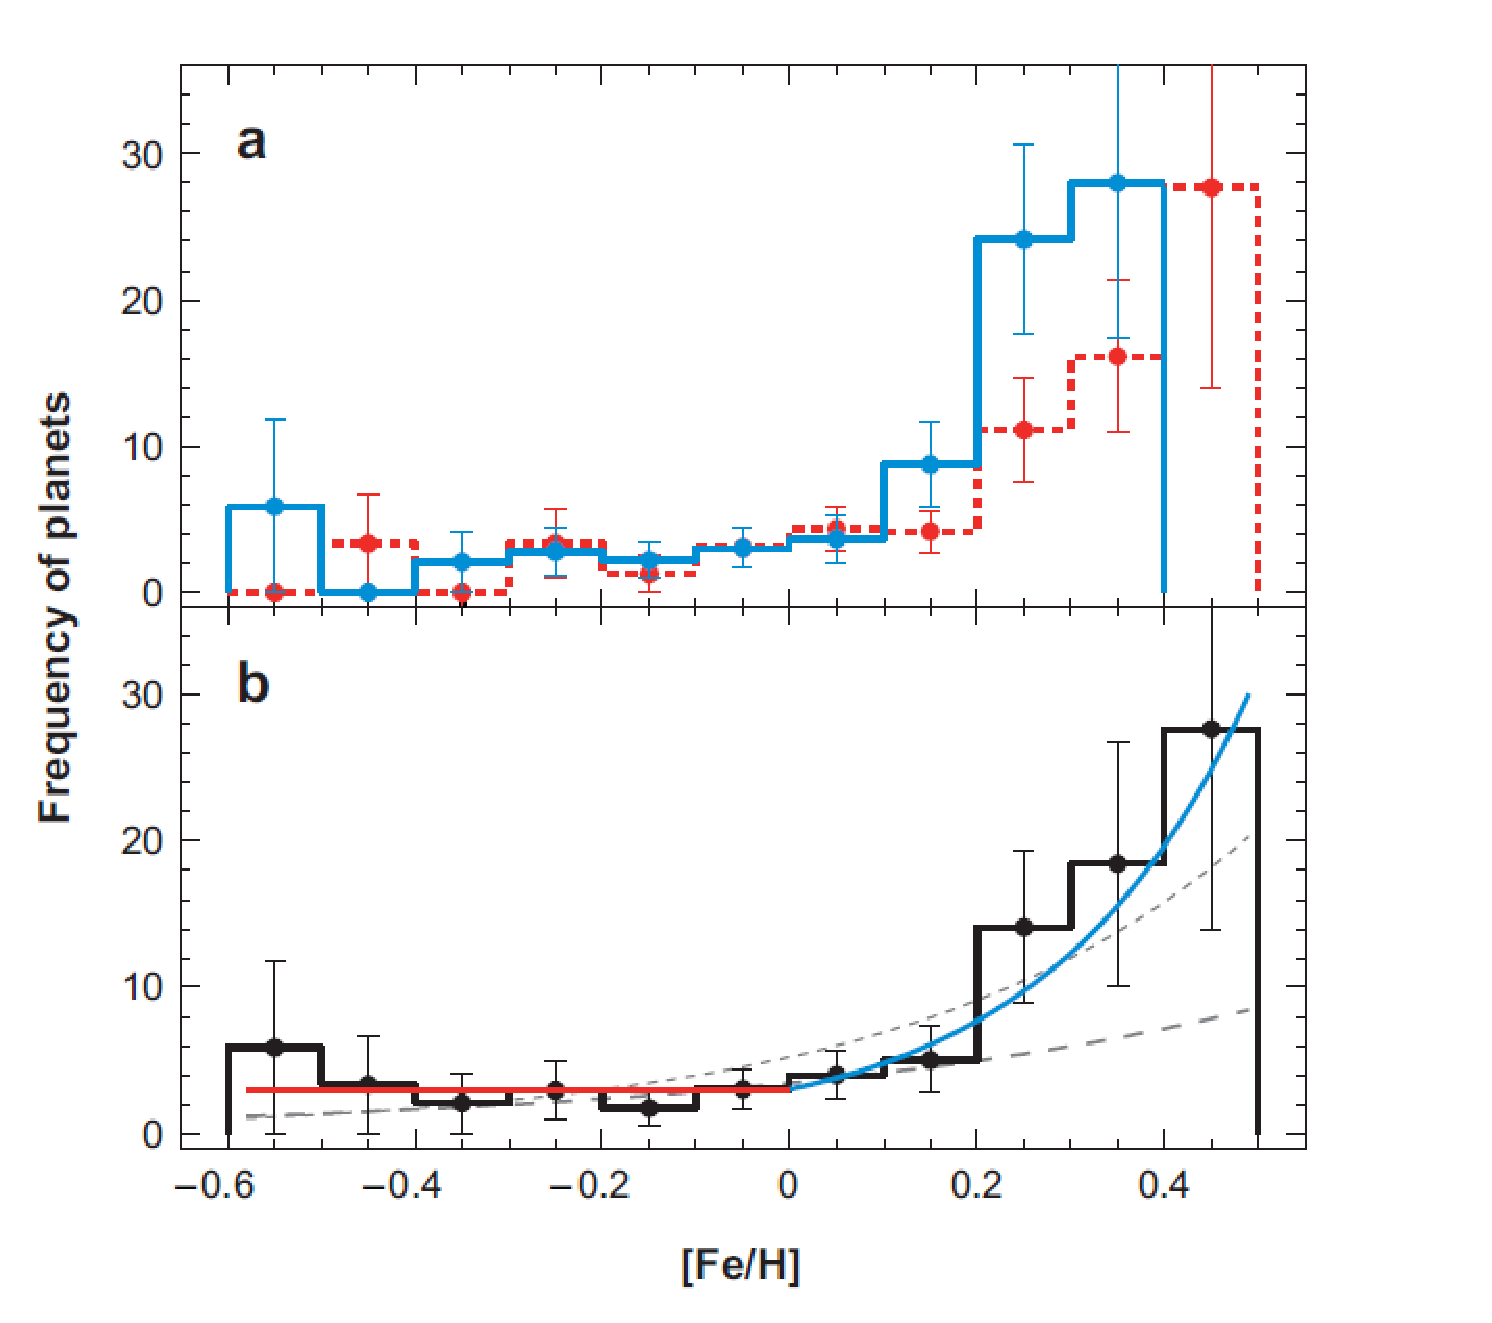
\includegraphics[height=9.3cm]{pics/fehhist.eps}
\caption[] {a) Percentage of planet hosts with stellar metallicity from CORALIE (blue) and Lick-Keck (red) samples. The lowest metallicity part of the histogram has few planet hosts and therefore its statistics are poor.; b) Average distribution of the two samples. The blue curve represents a power law fit of the data using only the [Fe/H] values greater than 0.0. The red line represents an average value for [Fe/H] between -0.5 and 0.0. From \citet{Udry-2007}.}
\label{fehhist}
\end{figure}



\citet{Woolf-2005} studied 35 M and K dwarfs using the classical approach of calculating metallicities measuring atomic line equivalent widths (EWs) from high-resolution spectra. The lines of Iron were chosen very carefully from regions clean of molecular lines \citep{Woolf-2004}. This work was later expanded to 84 stars \citep{Woolf-2006}. However, this method can only give reliable metallicities in relatively hot stars ($T_{eff}> 3500K$) with low metallicities ( [Fe/H] between -2.4 and +0.2 dex). This is due to the fact that cooler and more metal rich stars have a greater influence of molecular lines in their spectra. Despite that, the same authors, in \citet{Woolf-2006}, use these results to create a metallicity calibration with molecular indices, namely CaH2, that is well correlated with effective temperature, and TiO5, both correlated with temperature and metallicity (Fig. \ref{ww06bon05}a). These indices can be calculated with low resolution spectra ($\lambda/\Delta\lambda\sim3000$), which allows the measurement of metallicity on fainter and/or farther M stars. The bounds of the calibration extend from [Fe/H] values of +0.05 to -1.0 with a limited extension to -1.5 dex, having an estimated uncertainty of $\pm0.30$ dex. %Despite that, there is no  published quantitative relation to calculate the metallicity.


\begin{figure}[h]
\centering
%\subfigure[]{
\includegraphics[height=5 cm]{pics/branco}}
\subfigure[]{\includegraphics[height=6 cm]{pics/ww06_2.eps}}
\subfigure[]{\includegraphics[height=6 cm]{pics/bonfils05.eps}}
\caption[] {a) Equal metallicity contours in the plot of the indices CaH2 vs. TiO5. From \citet{Woolf-2006}; b) Color-magnitude diagram $V-K$ vs $M_{K}$ . The filled circles correspond to the metallicity determinations of \citet{Bonfils-2005} and the open circles to those from\citet{Woolf-2005}. The symbol size is proportional to the metallicity. The dashed lines represent isometallicity contours spaced by 0.25 dex from $-1.50$ dex (left) to $+0.25$ dex (right). The right hand axis shows masses from the \citet{Delfosse-2000} K-band mass-luminosity relationship, which has very low dispersion and allows to interpret the figure as a mass-colour-metallicity diagram. From \citet{Bonfils-2005}.}
\label{ww06bon05}
\end{figure}


Other attempts to calibrate the metallicity on M dwarfs have been done using binaries where an M dwarf is the secondary of a FGK star. In these cases, the metallicity is inferred from the hotter primary by high resolution spectral analysis.  \citet{Bonfils-2005} used this technique to calculate metallicities for 20 M dwarf secondaries, together with the metallicities from a set of \citet{Woolf-2005} sample, to create a photometric calibration (see Fig. \ref{ww06bon05}b). The calibration is valid for $M_{k}$ between 4 and 7.5, $V-K$ between 2.5 and 6, [Fe/H] between -1.5 and 0.2 dex, and needs V-band, K-band photometry, and accurate parallaxes from the Hipparcos sattelite \citep{Perryman-1997}. The uncertainty of the calibration is approximately 0.20 dex and only for stars closer than $\sim$ 50 pc, due to the parallax limitation. The results of \citet{Bonfils-2005} are intriguing. In their study, the mean metallicity of M dwarfs with planets is [Fe/H] = -0.11 dex %[recalculate this for M stars that exist now in 2010]
, while the FGK planet hosts have a mean metallicity of +0.15 dex (\citeauthor{Santos-2004b} \citeyear{Santos-2004b}; \citeauthor{Fischer-2005} \citeyear{Fischer-2005}). Moreover, they found that the metallicity of M dwarfs, using the calibration, in their complete, volume limited sample of FGKM dwarfs have a $\sim$0.07 dex shift toward lower metallicities. This may imply that the decreased frequency of Jovians around M dwarfs is a reflection of their lower metallicities rather than their lower masses. 

The high-resolution spectral synthesis technique is also starting to produce its first important results for M dwarfs (e.g. \citeauthor{Valenti-1998} \citeyear{Valenti-1998}; \citeauthor{Bean-2006} \citeyear{Bean-2006}). Basically, the technique consists on using a model atmosphere program like PHOENIX (e.g \citet{Hauschildt-1999}) and a stellar analysis program that is able to synthesize spectra, like SYNTH \citep{Piskunov-1992} or MOOG \citep{Sneden-1973}. In the end, the synthetic spectra atomic or/and molecular lines are fitted to the observed ones in order to extract the stellar parameters (Fig. \ref{bean06}). 
%(typically the effective temperature, surface gravity, metallicity, microturbulence). 
 \citet{Bean-2006} used this technique to determine with precision the stellar parameters of M dwarfs. He found that his results were consistent to 0.11 dex with techniques applied to solar-type stars, with uncertainties of 48 K, and  0.12 dex for effective temperature, and metallicity, respectively. These uncertainties do not include any kind of systematic errors, and the models do not reproduce all the features of the complex M dwarf spectra. Therefore all results should be taken with care. This technique was applied later on by \citet{Bean-2006b} to determine the metallicities of three planet host stars. It was found that all stars have subsolar metallicities, which contrasts strongly with the observed trend seen in FGK hosts, and have even lower, however compatible, values than those of \citet{Bonfils-2005}.

\begin{figure}[h]
\centering
\includegraphics[height=9cm]{pics/bean2006b.eps}
\caption[] {Spectral region near a strong TiO band head of GJ 876. The best fit used to determine the stellar parameters is over- plotted (solid black line). For comparison, synthetic spectra computed with metallicity values 0.3 dex lower (dotted line) and higher (dashed line) than the best-fit value are also overplotted. From \citet{Bean-2006b}.}
\label{bean06}
\end{figure}

A completely different technique was devised by \citet{Casagrande-2008}, based on his previous study of FGK stars using the infrared flux method (IFRM; \citeauthor{Casagrande-2006} \citeyear{Casagrande-2008}) to determine effective temperatures and metallicities. The infrared flux method is a technique that uses multiple photometry bands to derive effective temperatures, bolometric luminosities, and angular diameters of the star. The basic idea of IRFM \citep{Blackwell-1977} is to compare the ratio between the bolometric flux and the infrared monochromatic flux, both measured at Earth, to the ratio between the surface bolometric flux ($\propto\sigma Teff^{4}$) and the surface infrared monochromatic flux of the star. In order to adapt this method to M dwarfs, new optical bands were added, creating the so-called MOITE, Multiple Optical and Infrared TEchnique. This new technique provides very sensitive indicators of both temperature and metallicity, with the proposed effective temperature scale extending down to 2100-2200 K, into the L-dwarf limit, being supported by interferometric angular diameters above $\sim$ 3000K. However, new studies are needed to confirm the effective temperature measurements, especially below 3000 K. Regarding the metallicities, they are in very good agreement with the ones calculated by \citet{Bonfils-2005}, \citet{Woolf-2006}, and \citeauthor{Bean-2006} (\citeyear{Bean-2006},\citeyear{Bean-2006b}). A test using M dwarfs in binaries with FGK stars, suggest that the metallicities are reliable even below 3000K. This allows the opening of galactic chemical evolution investigations to ultra-cool stars. The internal uncertainties of the effective temperature is of the order of $\sim$50 K, and $\sim$0.2 dex for [Fe/H] within 1.5$\sigma$. The total uncertainty of the metallicity is estimated to be between $\pm$0.2 and $\pm$0.3 dex, and the external uncertainty for effective temperatures below 3000 K is of the order of $\sim100 K$.  %Regarding the calculated M star radii, the estimated error is of the order of 6\%, and it agrees, in general, with interferometric determined radii. 
The next step will be to use this calibration to study the parameters of M dwarfs with planets.

% NOTE - Bonfils calibration was used in Casagrande 2008 as starting point for calculating feh!!!! VERY IMPORTANT!
% NOTE - ver 7.1 do Casagrande 2008 para escrever sobre determinacao de raio da estrela

More recently, \citet{Johnson-2009} tested the \citet{Bonfils-2005} calibration. They created an empirical model using a color-magnitude diagram, in which the vertical distance of the M dwarf to the mean metallicity of the main sequence M stars, assumed as equal to the mean metallicity of a volume limited sample of FGK stars from the SPOCS sample \citep{Valenti-2005}, is a measure of the star metallicity (Fig. \ref{ja09sl10}a). They also added from this sample 6 M dwarfs with wide high metallicity FGK companions. From their calibration, they found out that the metal rich stars of \citet{Bonfils-2005} are systematically underestimated, by an average of 0.32 dex, attributing this to a lack of metal rich stars in their sample, or due to the use of poor V magnitudes. They conclude that M dwarf planet hosts follow the same trend as FGK stars, that is, they are preferentially metal rich. They also suggest that the lack of Jovian planets around M dwarfs is mostly correlated to a lower stellar mass and not to a lower value of [Fe/H], being more consistent with the works of planetary formation around M stars (i.e. \citeauthor{Laughlin-2004} \citeyear{Laughlin-2004}; \citeauthor{Ida-2005} \citeyear{Ida-2005}). The calibration of \citet{Johnson-2009} is valid for $V-K$ values between 3.9 and 6.6 mag. 

\begin{figure}[h]
\centering
\subfigure[]{\includegraphics[height=6 cm]{pics/JA09.eps}}
\subfigure[]{\includegraphics[height=6 cm]{pics/SL2010.eps}}
\caption[] {a) Nearby low-mass stars in the {$V - K$ , $M_{K}$ } plane. The small black circles represent a volume-limited sample of single K dwarfs ($M_{K} \leq 5.5$, d < 20 pc) and M dwarfs (d < 20 pc). The solid line is a fifth-order polynomial fit to the mean MS. The dashed lines are the isometallicity contours from the \citet{Bonfils-2005} photometric metallicity calibration. The large red circles are the positions of a sample of high-metallicity M dwarfs, with spectroscopic [Fe/H] measured from their FGK binary companions. The $V - K$ colors of various spectral types are listed at the bottom of the figure. From \citet{Johnson-2009} ; b) Optimally-smoothed residual distributions for \citet{Bonfils-2005} and \citet{Johnson-2009}. In both cases the vertical dashed line indicates the mean of the distribution. Note that the \citet{Bonfils-2005} distribution has a heavy tail at large positive values (indicating systematically low [Fe/H] estimates) and the \citet{Johnson-2009} distribution has a heavy tail at large negative values (indicating systematically high [Fe/H] estimates). From \citet{Schlaufman-2010}.}
\label{ja09sl10}
\end{figure}



Following the work of \citet{Johnson-2009}, \citet{Schlaufman-2010} created a vey similar calibration but with two major differences: first, they used an alternative set of M dwarfs: a complete, volume-limited and kinematically matched sample to calculate the mean M dwarf main sequence metallicity, the Geneva-Copenhagen survey (GCS - \citeauthor{Nordstrom-2004} \citeyear{Nordstrom-2004}). They claim that this catalogue is  more unbiased and outlier-sensitive when compared to other catalogues. Therefore, the mean MS metallicity value for the M dwarfs is -0.14, as opposed to -0.05 dex of \citet{Johnson-2009}; second, they used the \citet{Baraffe-1998} models to determine in which direction on the $V-K_{s}$, $M_{Ks}$ plane the [Fe/H] changes, concluding that metallicity should best correlate with horizontal shifts in the mentioned plane. For this reason, they compute the distance from the M dwarf main sequence to the M dwarf star only in the horizontal direction. Afterwards, they created a new calibration, concluding that the previous empirical photometric calibrations systematically underestimate \citep{Bonfils-2005} or overestimate \citep{Johnson-2009} metallicity at the extremes of their range (see Fig. \ref{ja09sl10}b). The uncertainty of the calibration is not mentioned: instead, they compute a multiple correlation coefficient, $R$, claiming that their model is one order of magnitude better in explaining the variance in the calibration sample than previous studies (i.e. $R  \sim$ 0.49 for their model, 0.06 for \citeauthor{Johnson-2009} \citeyear{Johnson-2009}, and 0.05  for \citeauthor{Bonfils-2005} \citeyear{Bonfils-2005}). In the end, they conclude that their results suggest that metal rich M dwarfs are more likely to host planets, as in FGK stars, and they claim that there is a hint that this correlation might extend to low-mass planets as well. This last result is in opposition to results obtained for low-mass planets orbiting FGK stars, which state that there is no significative relation between metallicity and the existence of low-mass planets. 



Finally, \citet{Rojas-Ayala-2010} recently released a new paper describing a novel and very precise technique that allows an easier observation of late type M dwarfs as well as farther, fainter, stars. Their technique is based on the calculation of spectral indices via direct spectral analysis of moderate (R $\sim2700$) near infrared spectra (K band), and has the advantage of not depending on V magnitudes nor parallaxes, allowing the study of fainter (or/and farther) stars. They analysed 17 M dwarfs secondaries with a FGK primary, that served also as metallicity calibrators, and measured the EWs of the NaI doublet (2.206 and 2.209 $\mu m$), and the CaI triplet (2.261, 2.263 and 2.265 $\mu m$). With these measurements and a water absorption spectral index sensitive to stellar temperatures, they constructed a metallicity scale (see Fig. \ref{RA10}) with an adjusted multiple correlation coefficient greater than the one of \citet{Schlaufman-2010} (R $\sim$ 0.63), and also with a tighter \textit{RMS} of 0.02 when compared to other studies (0.05, 0.04 and 0.02 for \citet{Bonfils-2005}, \citet{Johnson-2009}, and \citet{Schlaufman-2010} respectively). The water index was also used to diagnose the spectral types of the stars. The metallicity range of the calibration is between -0.5 and +0.5 dex, with an estimated uncertainty of $\pm$0.15 dex. Their results agree with \citet{Johnson-2009} and \citet{Schlaufman-2010} that M dwarf planet hosts appear to be systematically metal rich, a result consistent with the [Fe/H] distribution of FGK stars with planets. Neptunian host stars also seem to follow the trend of FGK stars, having a lower metallicity than Jovian hosts.%, and having a similar metallicity of the MS FGK stars.

\begin{figure}[h]
\centering
\includegraphics[height=9cm]{pics/RA2010.eps}
\caption[] {A linear combination of the EWs of the Ca I and Na I features versus the H2O-K index for the M dwarf sample. The big red and blue dots are M dwarfs in our metallicity calibration sample with $[Fe/H]>-0.05$ and $[Fe/H]<-0.05$, respectively. The small red and blue dots represent M dwarfs with $[Fe/H] > -0.05$ and $[Fe/H] < -0.05$ respectively, according to the photometric calibration by \citet{Johnson-2009}. The big black dots represent the M dwarf planet hosts. The dashed lines in the top panel are iso-metallicity contours. From \citet{Rojas-Ayala-2010}.}
\label{RA10}
\end{figure}



\subsection{Mass \& Radius}

The mass and radius determination are usually estimated using stellar evolutionary models, such as \citet{Baraffe-1998}. However, the models need very precise observational data as input, such as effective temperature, surface gravity, and metallicity from high-resolution spectral analysis. 

Masses can also be determined by empirical mass-luminosity relationships, the best of which is from \citet{Delfosse-2000}, where the relationship between infrared absolute magnitude and mass is very tight, beyond measurement errors (Fig. \ref{delfosse2000}). From here, \citet{Delfosse-2000} created a few very tight empirical calibrations for the mass. However, the calibrations are magnitude limited (for instance, $M_{k}$ is between 4.5 and 9.5). Nevertheless, the agreement with evolutionary models is excellent. The determinations have an accuracy between 0.2 to 10\% (with most of the error due to uncertainties in the parallaxes). 

\begin{figure}[h]
\centering
\includegraphics[height=7cm]{pics/Delfosse2000.eps}
\caption[] {K-band Mass-Luminosity relationship. From \citet{Delfosse-2000}.}
\label{delfosse2000}
\end{figure}

Regarding direct mass and radii determinations, the published measurements in the literature are not abundant. The eclipsing binary technique is capable of measuring M dwarf radius and mass with an accuracy of 1-10\%. However, the systems with eclipsing binaries are rare, and there are only eight known systems with a M star secondary, according to \citet{Ribas-2006}. In the last few years, it was possible to finally measure the radii of low mass stars with interferometry, with an accuracy of 1-5\%. There are at least 16 such measurements (e.g. \citeauthor{Segransan-2003} \citeyear{Segransan-2003}; \citeauthor{Demory-2009} \citeyear{Demory-2009}). At first, a large discrepancy (10-15\%) between observed and predicted radii was observed, as pointed out by \citet{Ribas-2006} and confirmed by \citet{Casagrande-2008}, using the MOITE technique (that can also be used to determine stellar radii). %(but, in this last case, only in the transition region between K and M stars). 
However, the work of \citet{Demory-2009} shows that this does not happen for almost all M dwarfs measured by interferometry, attributing the radii inflation to the fact that all members of eclipsing binaries are magnetically active fast rotators, as demonstrated theoretically by \citet{Chabrier-2007}, and clearly showing that there is an excellent agreement between predicted and measured radii for interferometric measurements.

When a precise determination of stellar mass and radius is achieved, it can be used for the derivation of precise planetary parameters (mass, radius, and mean density), providing that data from a photometric transit signal is available \citep{Torres-2008}. 

\subsection{Surface Gravity}

Surface gravity is calculated with precision in studies of high resolution spectral analysis, either directly or by means of synthetic to observational spectra fitting (e.g. \citeauthor{Woolf-2005} \citeyear{Woolf-2005}; \citeauthor{Bean-2006} \citeyear{Bean-2006}, respectively). However, it seems to be disregarded in the majority of other studies, where they input it as a fixed value, usually 5.0 dex, arguing that the effect of varying it $\pm$ 0.5 dex implies only minor differences to the other parameters (e.g. \citeauthor{Casagrande-2008} \citeyear{Casagrande-2008}). Direct measurements have been done by \citet{Fernandez-2009}, with eclipsing binaries, and \citet{Demory-2009}, with interferometry, obtaining a value of $\sim$ 4.9 dex and between 4.6 and 4.9 dex, respectively. However, the measurements are limited only to a handful of stars.

%\subsection{Planetary Mass and Radius}

%The precise determination of stellar mass and radius is critical for the derivation of precise planetary parameters (mass, radius, and mean density), providing that data from a photometric transit signal is available (\citet{Torres-2008}. Stellar Radii can be measured directly, by interferometry, but there are only a handful of measurements today, and new measurements are not easy to obtain. Therefore, the best practical way consists in applying a good technique to derive precise stellar parameters (effective temperature, surface gravity, metallicity) and use them as input in detailed stellar evolutionary models in order to obtain the stellar masses and radii. Alternatively one can use the excellent empirical mass determination relationships of \citet{Delfosse-2000} or/and the radii determinations of \citet{Casagrande-2008}.


%meter 2 paragrafos finais. Um sobre o raio (ver paper casagrande), outro sobre a massa (ver delfosse 2000), ver resumo parte SL10 acho
% referencias mass - delfosse 200 (MLR), baraffe 1998 (model for radii and mass), torres 2008 (for transits - see resume of nuno), 

%NOTE : I don't understand why they refer the synthetic spectra if they did not use it!!!




%Regarding logg most of the studies seem to disregard its importance, usually inputing 5.0 dex as an unique value for all M dwarfs. They say that a change in $\pm$0.5 dex in the surface gravity implies only minor differences in the derived parameters.

%ver teff scale for Reid&Hawley 2005 [from Casagrande 2008]

\section{Objectives}

The general goal of this thesis is to develop new tools to allow the determination of stellar parameters (especially effective temperature and metallicity) and chemical abundances in M dwarfs. In order to achieve this, different strategies will be developed, using low and high-resolution spectra, as well as photometric, interferometric and astrometric data, among others. Once these parameters are derived, they will be used to study the star-planet connection, looking for correlations between planetary (mass, radius, period, eccentricity...), and the stellar parameters. With the help of data from the transit technique, it will be also possible to refine the planetary parameters, radius and mass, and consequently, to calculate their mean density, thus allowing to have a first insight into the composition of extra-solar planets, by comparing this data to models of planetary formation and evolution (\citeauthor{Ida-2004b} \citeyear{Ida-2004b}; \citeauthor{Mordasini-2009} \citeyear{Mordasini-2009}).

In order to achieve this goal, I intend to work on my research from the following guidelines:  

\begin{itemize}

\item Use already available spectra of FGK dwarfs in binary systems where the secondary star is an M dwarf (also with available spectra) to characterize the metallicity and chemical abundances of the M star.

\item Use the derived values, together with the M dwarf spectra, to study spectral regions that may be particularly sensitive to any of the stellar parameters and to variations in the chemical abundances of these stars.

\item Use chosen spectral regions, clean of molecular lines, to measure the EWs of atomic /molecular lines, or/and calculate molecular indices, in order to directly determine the stellar parameters (especially, effective temperature and metallicity).

\item Use online databases to search for stellar spectroscopic, photometric, interferometric and astrometric data relevant for the work in progress. 

\item Update atomic and molecular line-lists to allow for a better computation of synthetic spectra for cool stars. Use the latest atmospheric models for cool stars together with radiative transfer codes, to produce a library of synthetic spectra for cool M dwarfs. 

\item Compare synthetic and observational spectra of M dwarfs to derive their parameters, including metallicity and chemical abundances. 

\item Submit telescope time proposals (ESO and other) to obtain low and high resolution spectra, and photometry of M dwarfs in different spectral ranges (optical and infra-red). %[e n�o s�...]. 

\item With the obtained values of metallicity and other data, establish a high-precision metallicity scale for M dwarfs. Use this scale to search for planet-metallicity correlations and to disentangle the dependence of the stellar mass from the stellar metallicity regarding the exoplanet formation. The final objective is to find correlations down to the regime of super-Earth planets.

\item Derive better planetary parameters for the orbiting planets, with the aid of data from transits. 

\end{itemize}

%NOTA - Item3. How will I update the atomic and molecular line lists?!??

\section{Methods}

In this section, I will give a brief overview of the methods I intend to use or improve during the course of my Ph.D.  It is always important to note that, perhaps, the best methods might have not been created yet, but they will emerge from those that already exist. This chapter will roughly go through the objectives guidelines, following closely the state of the art.

\subsection{Metallicity calibration with FGK+M binaries}

The first and the most accessible method I will try, at this time, involves the spectral analysis of high-resolution spectra of FGK primary stars with an M dwarf secondary. The stellar parameters of the primary are calculated following the method of \citet{Santos-2004b}, by imposing excitation and ionization equilibrium. A grid of Kurucz model atmospheres \citep{Kurucz-1993} is used in this process, as well as the radiative transfer program MOOG \citep{Sneden-1973}.The metallicity of the secondary is inferred from the obtained value of the primary. I will then use these values to update the metallicity calibration done by \citet{Bonfils-2005}, and compare it to the more recent calibrations as well, such as \citet{Casagrande-2008}, \citet{Johnson-2009}, \citet{Schlaufman-2010}, and  \citet{Rojas-Ayala-2010}. To this end, I will also need very precise visual and infrared photometry, and precise parallaxes. This approach has the advantage of using proven methods of calculating metallicities that are very precise and reliable. However, it is only possible to calculate the [Fe/H] for the companion M dwarf. Moreover, it is an infered value, not a direct one. The visual photometry will be obtained from different databases, that can be found, for instance, in Vizier \citep{Ochsenbein-2000}, and the infrared photometry will be taken from 2MASS \citep{Skrutskie-2006}. The parallaxes will be taken from the new reduction of the raw data of Hipparcos \citep{van_Leeuwen-2007}. An extension of this calibration is foreseen, with metallicity derived from the cross correlation function (CCF, \citeauthor{Santos-2002a} \citeyear{Santos-2002a}) of planet search programs such ELODIE \citep{Baranne-1996}, CORALIE \citep{Queloz-2000c}, SOPHIE \citep{Bouchy-2006}, and HARPS \citep{Pepe-2002}. 

\subsection{Direct Spectral Analysis}

The next step will not be so straightforward, as there are various routes one can take. One of the possibilities is to search for spectral regions in M dwarf spectra sensitive to stellar parameters, especially, effective temperature and metallicity. In these regions I'll try to find atomic or molecular lines in clean areas of the spectra, that is, without contamination of very weak molecular line bands, that are characteristic of M dwarfs. Afterwards, a classical spectral analysis may be done, similar to the one for hotter FGK stars, but with updated atmospheric models for M stars, namely the ones based on the PHOENIX model atmospheres\footnote{\url{http://perso.ens-lyon.fr/france.allard/}}$^{,}$\footnote{\url{http://www.hs.uni-hamburg.de/EN/For/ThA/phoenix/index.html}}  \citep{Allard-1995}. A direct spectral analysis will be based on the work of authors such as  \citet{Woolf-2005}, and \citet{Rojas-Ayala-2010}. The big advantage of this technique is that one does a direct spectral analysis with the potential of giving very precise values of the stellar parameters, such as effective temperature, surface gravity, micro-turbulence and metallicity all at once. The drawback is that the atmospheric models are not as reliable as the ones for hotter stars yet. The pseudo-continuum of the spectra might be badly estimated, giving, in the end, the wrong value for the parameters. The choice of the spectral area is critical for this. Another disadvantage is that it is only possible to get high resolution spectra for the nearest M dwarfs due to their intrinsic faintness.

Alternatively, one can find regions with some well-defined molecular bands and use it to create spectral indices, dependent on temperature or/and metallicity. This indices are defined as the ratio between the strength of the spectral feature and the strength of the 'pseudo-continuum' (e.g. \citeauthor{Gizis-1997} \citeyear{Gizis-1997}). Using indices is useful in spectra where it is not possible to make absolute measurements of the strength of the features, as it is the case of late type M dwarfs. The indices might also have the advantage of giving reasonable measurements when used in lower resolution spectra to calculate parameters in fainter or/and farther M stars. However, the results with lower resolution spectra tend to be less precise, with a rougher estimation of these quantities. Research on spectral indices will be based on the works of \citet{Woolf-2006}, \citet{Woolf-2009}, and \citet{Rojas-Ayala-2010}. 

\subsection {Synthetic spectra analysis}

Another possible route to extract the stellar parameters is to fit high resolution synthetic spectra to observed spectra. Until recently, the model atmospheres used to make the synthesis lacked the appropriate opacities and molecular transitions in order to reproduce the fine details of high resolution spectra (e.g. \citeauthor{Valenti-1998} \citeyear{Valenti-1998}). However, models are evolving very fast and they now incorporate several hundred millions of atomic and molecular line opacities, allowing the extraction of the stellar parameters, like effective temperature, surface gravity, microturbulence and metallicity with reasonable precision. It might be possible that this technique can be used to reach a better precision than direct spectral analysis in the next few years. In order to conduct my research, I'll use the synthetic spectra based on the latest models, such as the ones based on the PHOENIX code\footnote{\url{http://phoenix.ens-lyon.fr/simulator/index.faces}},  as well as the latest studies on this topic (e.g. \citeauthor{Bean-2006} \citeyear{Bean-2006}; \citeauthor{Bean-2006b} \citeyear{Bean-2006b}). 

\subsection {The MOITE technique}

The MOITE technique of \citet{Casagrande-2008} might also be very interesting to work with and improve. It relies only on multi-band infrared and optical photometry, but uses the latest PHOENIX model atmospheres  to compute the small part of the flux which is outside the observational bands, in order to calculate the bolometric flux. A basic description of this technique is detailed on Section 2.1. The obtained precision for effective temperature and metallicity is similar to other methods, with the claimed advantage that the metallicities are valid down to 2100-2200 K. The obvious way to improve this method is to obtain even more precise optical (BVRI) and infrared (JHK) photometry. However, it is hard to obtain or measure ultra-precise photometry for many stars, especially for fainter M dwarfs. It is also possible to determine accurate radii using this technique, which agrees up to 6\% with interferometric measurements.

\subsection {Stellar and planetary mass/radius determination}

The determination of mass and radius, for the moment, will be achieved either by using stellar evolution models for M dwarfs, such as \citet{Baraffe-1998} with input from direct spectral analysis/spectral synthesis or by using the empirical mass-luminosity relationship of \citet{Delfosse-2000} (for mass) and the \citet{Casagrande-2008} method (for radii). Alternatively, one can also use the radii provided by interferometry, provided that there is a significant increase of these kind of measurements. Afterwards, this information can also be used to refine the planetary mass and radius with the aid of data coming from photometric transits \citep{Torres-2008}.





%MAIL - 





%IDEIAS: look for spectral regions correlated with parameters especially, teff, and feh.; use the latest models of synthetic spectra ; look for other methods, like MOITE. 
%ver ponto 3 do casagrande 2008 para surface gravity. ver tamb�m rojas-ayala pag 6, 3 paragrafo



%ideias para esta secccao - seguir os items e ir falando dos metodos segundo o que esta no state of the art.



\bibliographystyle{aa}
\newpage
\addcontentsline{toc}{chapter}{Bibliography}
\bibliography{mylib}

\end{document}

%FIGURAS%%%%%%%%%%%%%%%%%%%%%%%
%%%%%%%%%%%%%%%%%%%%%%%%%%%%%%%
\begin{figure}[h]
\begin{center}$
\begin{array}{cc}
\includegraphics[scale=0.25]{figs/} &
\includegraphics[scale=0.25]{neptune_v16_1_100_10d6_exc_PT_1930PL.eps}
\end{array}$
\end{center}
\caption[Varia��o da excentricidade de Plut�o.]{Gr�fico da varia��o da excentricidade de Plut�o ao longo do tempo. A imagem da esquerda foi obtida para 300 mil anos e a imagem da direita para 10 milh�es de anos. A excentricidade m�dia � $\bar{e_1} \sim 0.24$.} \label{fig:exc1930PL}
\end{figure}

%DUVIDAS:

%please check mass and radius of the M dwarf (Chapter 1, paragraph 3, line 4)
%

